\documentclass{tufte-book}
\usepackage[T1]{fontenc}
\usepackage[utf8]{inputenc}
\title{Fizika  \thanks{Zahvaljujući vama.}}
\author[Google]{Mr. Fizičar}
\publisher{Učenicima srednjih škola}

\usepackage{pdfpages}
\usepackage{lipsum}
\usepackage{isotope}
\usepackage{booktabs}
\usepackage{titlesec}
\usepackage{graphicx}
\setkeys{Gin}{width=\linewidth,totalheight=\textheight,keepaspectratio}
\graphicspath{{multimedija/}}
\usepackage{mandi}
\usepackage{units}
\usepackage{amsmath,amsfonts,amsthm} % Math packages
\usepackage{mathtools}% http://ctan.org/pkg/mathtools
%\usepackage{mparhack}
\usepackage{sectsty} % Allows customizing section commands
\usepackage[dvipsnames]{xcolor}
\usepackage{pgf,tikz}
\usepackage{pgfplots}
\usetikzlibrary{shapes,arrows}
\usetikzlibrary{patterns,fadings}
\usetikzlibrary{arrows}
\usetikzlibrary{decorations.pathreplacing}
\usetikzlibrary{decorations.markings}
\usetikzlibrary{snakes}
\usetikzlibrary{spy}
\usepackage{setspace}
\usepackage{3dplot}
\usepackage{cancel}
\usepackage{physymb}
\usepackage{braket}
\usepackage{verbatim}
\usepackage{fancyvrb}
\fvset{fontsize=\normalsize}

\newcommand{\hangp}[1]{\makebox[0pt][r]{(}#1\makebox[0pt][l]{)}}

\newcommand{\hangstar}{\makebox[0pt][l]{*}}

\usepackage{xspace}
\usepackage{makeidx}
\makeindex

\newcommand{\vdqi}{\textit{VDQI}\xspace}
\newcommand{\ei}{\textit{EI}\xspace}
\newcommand{\ve}{\textit{VE}\xspace}
\newcommand{\be}{\textit{BE}\xspace}
\newcommand{\VDQI}{\textit{The Visual Display of Quantitative Information}\xspace}
\newcommand{\EI}{\textit{Envisioning Information}\xspace}
\newcommand{\VE}{\textit{Visual Explanations}\xspace}
\newcommand{\BE}{\textit{Beautiful Evidence}\xspace}

\newcommand{\TL}{Tufte-\LaTeX\xspace}


%\newcommand{\monthyear}{%
	%\ifcase\month\or January\or February\or March\or April\or May\or June\or
	%July\or August\or September\or October\or November\or
	%December\fi\space\number\year
%}
\usepackage{datetime}

\newdateformat{monthdayyeardate}{%
	\THEDAY. \THEMONTH. \THEYEAR. }

\newcommand{\openepigraph}[2]{%
	%\sffamily\fontsize{14}{16}\selectfont
	\begin{fullwidth}
		\sffamily\large
		\begin{doublespace}
			\noindent\allcaps{#1}\\% epigraph
			\noindent\allcaps{#2}% author
		\end{doublespace}
	\end{fullwidth}
}

\newcommand{\blankpage}{\newpage\hbox{}\thispagestyle{empty}\newpage}

\usepackage{units}

\renewcommand{\contentsname}{Sadržaj}
\renewcommand{\figurename}{Slika}
\renewcommand{\chaptername}{}
\newcommand{\measure}[3]{#1/#2$\times$\unit[#3]{pc}}

\newcommand{\hlred}[1]{\textcolor{Maroon}{#1}}% prints in red
\newcommand{\hangleft}[1]{\makebox[0pt][r]{#1}}
\newcommand{\hairsp}{\hspace{1pt}}% hair space
\newcommand{\hquad}{\hskip0.5em\relax}% half quad space
\newcommand{\TODO}{\textcolor{red}{\bf TODO!}\xspace}
\newcommand{\ie}{\textit{i.\hairsp{}e.}\xspace}
\newcommand{\eg}{\textit{e.\hairsp{}g.}\xspace}
\newcommand{\na}{\quad--}% used in tables for N/A cells
\providecommand{\XeLaTeX}{X\lower.5ex\hbox{\kern-0.15em\reflectbox{E}}\kern-0.1em\LaTeX}
\newcommand{\tXeLaTeX}{\XeLaTeX\index{XeLaTeX@\protect\XeLaTeX}}

% \index{\texttt{\textbackslash xyz}@\hangleft{\texttt{\textbackslash}}\texttt{xyz}}
\newcommand{\tuftebs}{\symbol{'134}}% a backslash in tt type in OT1/T1
\newcommand{\doccmdnoindex}[2][]{\texttt{\tuftebs#2}}% command name -- adds backslash automatically (and doesn't add cmd to the index)
\newcommand{\doccmddef}[2][]{%
	\hlred{\texttt{\tuftebs#2}}\label{cmd:#2}%
	\ifthenelse{\isempty{#1}}%
	{% add the command to the index
		\index{#2 command@\protect\hangleft{\texttt{\tuftebs}}\texttt{#2}}% command name
	}%
	{% add the command and package to the index
		\index{#2 command@\protect\hangleft{\texttt{\tuftebs}}\texttt{#2} (\texttt{#1} package)}% command name
		\index{#1 package@\texttt{#1} package}\index{packages!#1@\texttt{#1}}% package name
	}%
}% command name -- adds backslash automatically
\newcommand{\doccmd}[2][]{%
	\texttt{\tuftebs#2}%
	\ifthenelse{\isempty{#1}}%
	{% add the command to the index
		\index{#2 command@\protect\hangleft{\texttt{\tuftebs}}\texttt{#2}}% command name
	}%
	{% add the command and package to the index
		\index{#2 command@\protect\hangleft{\texttt{\tuftebs}}\texttt{#2} (\texttt{#1} package)}% command name
		\index{#1 package@\texttt{#1} package}\index{packages!#1@\texttt{#1}}% package name
	}%
}% command name -- adds backslash automatically
\newcommand{\docopt}[1]{\ensuremath{\langle}\textrm{\textit{#1}}\ensuremath{\rangle}}% optional command argument
\newcommand{\docarg}[1]{\textrm{\textit{#1}}}% (required) command argument
\newenvironment{docspec}{\begin{quotation}\ttfamily\parskip0pt\parindent0pt\ignorespaces}{\end{quotation}}% command specification environment
\newcommand{\docenv}[1]{\texttt{#1}\index{#1 environment@\texttt{#1} environment}\index{environments!#1@\texttt{#1}}}% environment name
\newcommand{\docenvdef}[1]{\hlred{\texttt{#1}}\label{env:#1}\index{#1 environment@\texttt{#1} environment}\index{environments!#1@\texttt{#1}}}% environment name
\newcommand{\docpkg}[1]{\texttt{#1}\index{#1 package@\texttt{#1} package}\index{packages!#1@\texttt{#1}}}% package name
\newcommand{\doccls}[1]{\texttt{#1}}% document class name
\newcommand{\docclsopt}[1]{\texttt{#1}\index{#1 class option@\texttt{#1} class option}\index{class options!#1@\texttt{#1}}}% document class option name
\newcommand{\docclsoptdef}[1]{\hlred{\texttt{#1}}\label{clsopt:#1}\index{#1 class option@\texttt{#1} class option}\index{class options!#1@\texttt{#1}}}% document class option name defined
\newcommand{\docmsg}[2]{\bigskip\begin{fullwidth}\noindent\ttfamily#1\end{fullwidth}\medskip\par\noindent#2}
\newcommand{\docfilehook}[2]{\texttt{#1}\index{file hooks!#2}\index{#1@\texttt{#1}}}
\newcommand{\doccounter}[1]{\texttt{#1}\index{#1 counter@\texttt{#1} counter}}



\begin{document}
	
	% Front matter
	\frontmatter
	
\includepdf{multimedija/fizika-intro}
	% r.1 blank page
	%\blankpage
	
	% v.2 epigraphs
	%\newpage\thispagestyle{empty}
	%\openepigraph{%
		%I think that modern physics has definitely decided in favor of Plato. In fact the smallest units of matter are not physical objects in the ordinary sense; they are forms, ideas which can be expressed unambiguously only in mathematical language.
%	}{Werner Heisenberg%, {\itshape Design, Form, and Chaos}
	%}
	%\vfill
	%\openepigraph{%
		%The only shibboleth the West has is science. It is the premise of modernity and it defines itself as a rationality capable of, indeed requiring separation from politics, religion and really, society. Modernisation is to work towards this\ldots If one looks at the works of Newton to Einstein, they were never scientists in the way modernity understands the term. 
%	}{Bruno Latour}
%\vfill
	%\openepigraph{%
		%The boundary between science fiction and social reality is an optical illusion.
%	}{Donna Haraway}
	
	
	% r.3 full title page
	\maketitle
	
	
	% v.4 copyright page
	\newpage
	\begin{fullwidth}
		~\vfill
		\thispagestyle{empty}
		\setlength{\parindent}{0pt}
		\setlength{\parskip}{\baselineskip}
		Copyright \copyright\ \the\year\ \thanklessauthor
		
		\par\smallcaps{Objavljeno \thanklesspublisher}
		
		\par\smallcaps{https://github.com/rumi55/Fizika}
		
		\par Licensed under the Apache License, Version 2.0 (the ``License''); you may not
		use this file except in compliance with the License. You may obtain a copy
		of the License at \url{http://www.apache.org/licenses/LICENSE-2.0}. Unless
		required by applicable law or agreed to in writing, software distributed
		under the License is distributed on an \smallcaps{``AS IS'' BASIS, WITHOUT
			WARRANTIES OR CONDITIONS OF ANY KIND}, either express or implied. See the
		License for the specific language governing permissions and limitations
		under the License.\index{license}
		
		\par\textit{Zadnja izmjena, \monthdayyeardate\today}
	\end{fullwidth}

	% r.5 contents
	\tableofcontents

	

	
	
	% r.9 introduction
	\cleardoublepage
	\chapter*{Napomena}
	
	Ova FIZIKA je projekat započet od strane učitelja fizike iz BiH koji su željni promjena.  Knjiga je pisana u \LaTeX \-u koristeći se otvorenim kodom \doccls{tufte-book} i \doccls{tufte-handout} za pisanje.  
	
	\vspace{2cm}
	
	https://github.com/rumi55/Fizika
	
	%%
	% Start the main matter (normal chapters)
	\begin{fullwidth}
		\chapter*{Predgovor}


	\section*{ ... }
	Treba napisati
	\section*{Kako se rješavaju zadaci?}
	Fizika predstavlja većini jedan od najstrašnijih predmeta u osnovnoj i srednjoj školi. Posebno takvom mišljenju doprinose zadaci, koje vrlo često ne znamo kako da počnemo. Ovaj tekst daće vam nekoliko glavnih smjernica za rješavanje zadataka iz fizike.
	
	Prvo i možda najvažnije pravilo jeste da se zadatak dobro pročita, s ovim dobro mislim na pažljivo i studiozno čitanje koje obično ide u tri etape. Prva etapa (ili prvo čitanje) je čisto da se informišemo  o čemu naš zadatak govori. Mnogi se plaše dugih zadataka, tj zadataka sa puno teksta, no obično su oni najlakši, jer sa puno teksta dolazi puno informacija koje nam kasnije pomažu da tak zadatak pravilno rijesimo.
	Druga etapa (čitanje) nam služi da zabilježimo sve podatke koje smo dobili u tekstu. Uobičajeno je  da se pišu jedan ispod drugoga, te da se na kraju povuče linija ispod koje pišemo šta se zapravo traži od nas da se uradi u tom zadatku. Treće čitanje (etapa) je vrlo važno, jer u njemu povezujemo sve podatke koje smo dobili.
	Kada smo završili sa iščitavanjem red je da se bacimo na rješavanje problema. Moj savjet je da se na papiru ispišu sve formule koje znamo, a da su relevantne za dati nam zadatak. Relevantne su one koje u sebi sadrže neke od podataka koje smo dobili, a pored toga moraju da odgovaraju i uslovima opisanim u problemu. Kad smo to uradili, sad je na nama da ih spojimo kao slagalicu. Da na jednoj strani imamo podatak koji se traži od nas, a na drugoj sve poznate informacije iz opisa zadatka.
	
	Ne zaboravite provjeriti cjelokupan zadatak još jednom, nakon proračuna. Provjerite rješenje i kompletan računski dio zadatka, jer se po pravilu uvijek potkrade neka sitna greška, koja nas  na kraju košta vrlo važnih bodova.
	Važno je istaći i to koliko sam rezultat ima smisla. Npr.  za rezultat ste dobili temperaturu sobe od 1000 stepeni celzijusa, ili automobil se kreće brzinom 3000 km na čas. Ovakve rezultati trebali bi da vas upozore da ste negdje pogriješili i da bi trebali još jednom da se vratite  kroz čitav zadatak.
	
	\begin{flushright}
		Autor
	\end{flushright}
	\newpage
	\pagenumbering{arabic}
	\patchcmd{\chapter}
	{\clearpage}
	{\cleardoublepage}
	{}
	{}
		\pagestyle{headings}
	\end{fullwidth}

	\mainmatter

	\section{Vektori}

		\chapter {Elektrostatika}


	\section{Uvodna razmatranja}
	U vrijeme antičke Grčke bile su poznate četiri pojave koje su povezane sa elektricitetom. To su munja, svjetlucanje oko šiljatih predmeta, ribe koje proizvode neku vrstu električnih udara i privlačenje laganih predmeta (slama) pomoću protrljanog komada ćilibara. Ove pojave su bile uočene, a sa elektricitetom povezane čitavih 2500 godina kasnije.

	\begin{marginfigure}%
		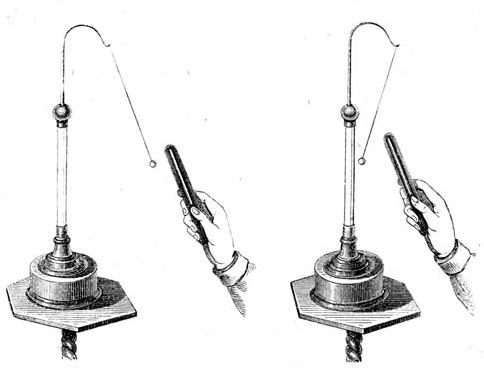
\includegraphics[width=\linewidth]{naboj}
		\caption{Naboj}
		\label{fig:naboj}
	\end{marginfigure}
	Aristotel (Aristotle, 384-322, pre n.e.) je opisao ribu torpiljarku ali nije uočio električni organ. Tales iz Mileta (Thalés Miléisos, oko 625-547. pre n.e.) je znao za privlačnu moć ćilibara koji su Sirijci zvali kamen kradljivac, a Perzijanci kradljivac slame (karuba). Grčki naziv elektor  ima značenje onaj koji privlači. U to vrijeme pominje se kamen linkurion, koji ima još veću moć privlačenja. Vjerovatno se radi o turmalinu ili topazu, jer se sa privlačenjem pominje i zagrijavanje kamena. U svim dokumentima iz tog perioda koji su sačuvani pominje se samo privlačenje. Odbojne sile tada nisu primijećene. Razlog za to je svuda prisutna gravitacija i znatno veće interesovanje za magnet koji privlači gvožđe, ma kako veliko bilo, dok ćilibar privlači različite, ali samo veoma lagane predmete. Takođe, pojava odbijanja nije mogla da se uklopi Aristotleovo učenje i učenje njegovih sljedbenika. Tek u šestom vijeku nove ere odbijanje kod magneta pominje Jovan Filopon. \\
	U periodu od 12, 13 vijeka Arapi su dali također veliki doprinos razvoju elektrostatike. U Evropi se značajnije pominje elektrostatia tek poslije.
	\begin{marginfigure}%
		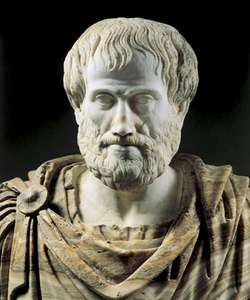
\includegraphics[width=\textwidth]{aristotle}
		\caption{Aristotel}
		\label{fig:aristotle}
	\end{marginfigure} 
	Naime, engleski ljekar Džilbert (William Gilbert 1544 – 1603) objavio je u svom djelu sistematsku raspravu o osobinama ćilibara da privlači vunu i rude magnetita da privlači gvožđe. On je Zemlju proglasio "velikim magnetom", 1630. godine je silu koja nastaje trenjem tijela nazvao \textit{vis electrica}.
	
	Za otkriće da elektricitet može da se kreće od jednog tijela do drugog zaslužan je Grej (Stephen Greu, 1670 – 1736), kao i za druge pojave. Godine 1733. došao je francuski fizičar de Faj (C. F. de Cisternay du Fay 1698 – 1739) do otkrića, da postoje dvije vrste elektriciteta, koje je nazivao staklasti i smolasti. 
	
	Tek 1975 godine je otkriven kondenzator u vidu staklene čaše sa naelektrisanim ekserom u njoj. Otkriće su predvodili Kleist i Mušenbruka. Ovaj eksperiment je ponovio Nole (Abbe Nollet) i dao ime uređaju Lajdenska boca. (Nikola Tesla: "Kleist i Mušenbruka su uspjeli da u bočicu zatvore tajanstvenu silu, koja iz bočice	bježi uz “ljuti” prasak, razvijajući rušilačku snagu. To je bilo rođenje kondenzatora, možda najčudesnije električne naprave koja je ikada pronađena").
	\begin{marginfigure}%
		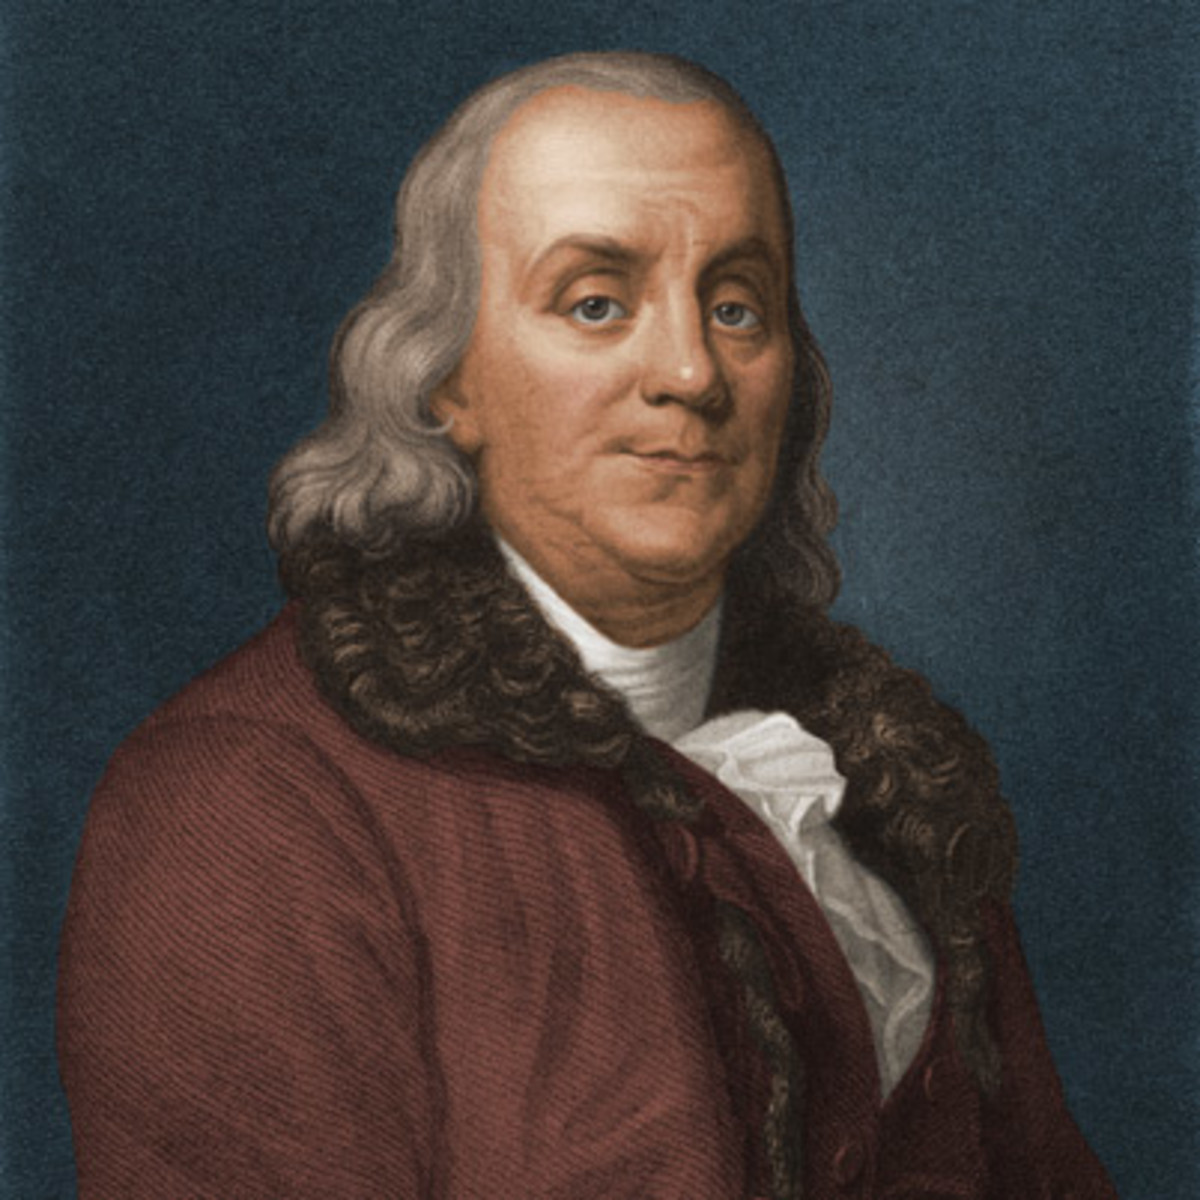
\includegraphics[width=\linewidth]{benjamin-franklin}
		\caption{Benjamin Frenklin}
		\label{fig:benjamin-franklin}
	\end{marginfigure} 
	Sjevernoamerički fizičar Benjamin Frenklin (1706 – 1790) je 1750. godine postavio
	prvu teoriju o prirodi elektriciteta: da je elektricitet fluid kojeg sva tijela imaju u određenoj količini. Benjamin Franklin je 1752. godine opisao grom kao električno pražnjenje i godinu kasnije pronašao gromobran. Godinu dana kasnije ruski fizičar Rihmen izvodio slične eksperimente, ali je prilikom toga poginuo od udara groma.\\
	Cijelo područje makroskopskih fenomena poznato pod nazivom elektrostatika osiguralo je istorijsku osnovu za razvitak koncepta elektrostatičkog naelektrisanja, kao mjerljive fizikalne veličine. Elektrostatika, jedno od glavnih područja nauke o elektricitetu, temelji se na samo jednom eksperimentalnom postulatu, inverznom kvadratnom zakonu, koji je jedan od fundamentalnih naučnih principa uopšte. Nije bio kreiran samo od jednog istraživača. 
	
	\begin{marginfigure}%
		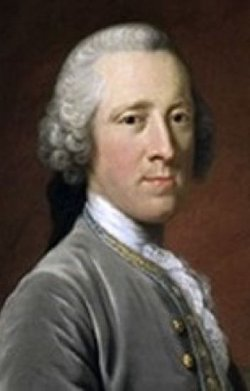
\includegraphics[width=\linewidth]{henry-kevendis}
		\caption{Henry Cavedish}
		\label{fig:kevendis}
	\end{marginfigure} 
	Prvi značajan doprinos dao mu je Benjamin Frenklin, a 1766. god. započeo je istraživanja Džozef Pristli (Joseph Priestley 1731 – 1804), na njegov podsticaj. Godine 1769. odredio je Robinson (J. Robinson 1739 – 1805) direktnim eksperimentom silu između električnih naelektrisanja, a Henri Kevendiš (Henry Cavendish 1731 – 1810) je 1773. definitivno potvrdio taj zakon. \\

	\begin{marginfigure}%
		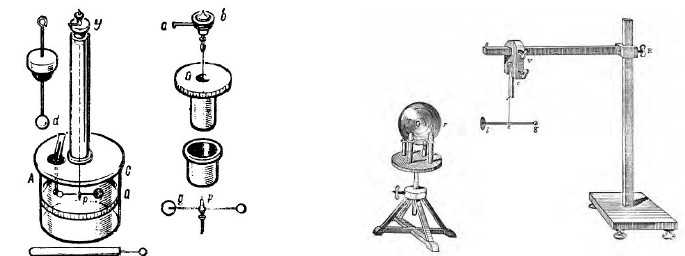
\includegraphics[width=\linewidth]{kulonova}
		\caption{Kulonova torziona vaga i uređaj za različita naelektrisanja}
		\label{fig:kulonova}
	\end{marginfigure}
	Kako je ustanovljeno da postoje dvije vrste naelektrisanja, pozitivno i negativno, što uslovljava privlačenje i odbijanje naelektrisanih tijela Kulon (Charles Augustin Koulon 1736 - 1860) je svojim radovima dao opšti zakon međusobnog djelovanja naelektrisanih tijela na nekom rastojanju. On je 1785. godine demonstrirao inverzni kvadratni zakon, pomoću precizne torzione vage, kojom mogu da se mjere veoma male sile. Ova vaga je dobila ime po njemu Kulonova torziona vaga.\\
	
	
	Njegova otkrića čine prvu kvantitativnu bazu za matematički prikaz zakona električne sile, koji utvrđuje da dva električno naelektrisana tijela, čija veličina je mala u odnosu na udaljenost između njih, djeluju jedno na drugo s jednakim i suprotnim silama, koje su obrnuto srazmjerne kvadratu njihove međusobne udaljenosti. Kulonova metoda eksperimentalnog određivanja inverznog kvadratnog zakona bila je direktna, kvantitativna i lahko razumljiva, pa su njegovi rezultati bili spremno prihvaćeni. To su prvi rezultati iz nauke o elektricitetu, koji su bili objavljeni i široko rasprostranjeni. \\
	\begin{marginfigure}%
		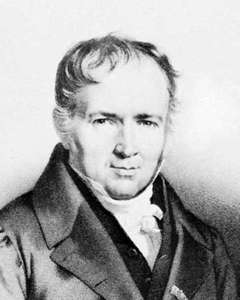
\includegraphics[width=\linewidth]{poisson}
		\caption{Simeon Denis Poisson 1781 – 1840}
		\label{fig:poisson}
	\end{marginfigure} 
	Tome su znatno	doprinijela i teoretska razmatranja S. Poasona, objavljena u dva memoara 1812. i 1813. godine. U njima je on, uzimajući Kulonov inverzni kvadratni zakon kao fundamentalni postulat, znatno unaprijedio i upotpunio elektrostatiku upotrebom analogije prema gravitacionoj teoriji, koja je tada bila visoko razvijena. S. Poason je, na osnovu Kulonovog zakona, uveo funkciju $ \Phi(x,y,z) $ , kojoj doprinose sva naelektrisanja jednog električnog sistema obrnuto proporcionalno s udaljenošću. Petnaest godina kasnije u generalisanju Poasonovih radova o električnim i magnetnim pojavama, Grin (1731 – 1841) daje funkciji $ \Phi $ univerzalno ime \textit{potencijal}.\\
	
		
		
	Voltin (Alessandro Volta 1745 – 1827) pronalazak prve hemijske baterije bio je neposredan podsticaj i za studij vođenja elektriciteta. Značajne rezultate u istraživanju vođenja postigli su Hamfri Dejvi (Humphry Davy 1778 – 1829) i Om (George Simeon Ohm 1787 – 1854). \\
	
	\begin{marginfigure}%
		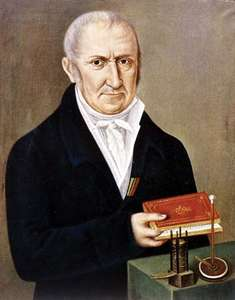
\includegraphics[width=\linewidth]{volta}
		\caption{Alessandro Volta}
		\label{fig:volta}
	\end{marginfigure} 

	Om je 1826. godine formulisao rezulta eksperimentalnih istraživanja, da je jačina struje u žici koja ne sadrži nikakvu elektromotornu silu proporcionalna razlici potencijala na njenim krajevima. Ta činjenica, iako ne spada u posebnu klasu zakona nezavisnih od materije, nazvana je Omovim zakonom. Zakon je u suštini vrlo jednostavan, no mora se upotrebljavati s pažnjom. Upravo zbog njegove jednostavnosti, trebalo je proći oko 14 godina, pa da to veliko otkriće u naučnom svijetu bude priznato i prihvaćeno. Godine 1841. Džul (J. P. Joule 1818 – 1889) utvrđuje zakon koji povezuje struju koja protiče metalnim provodnikom s razvijenom toplotom u njemu.\\
	
	
	\begin{marginfigure}%
		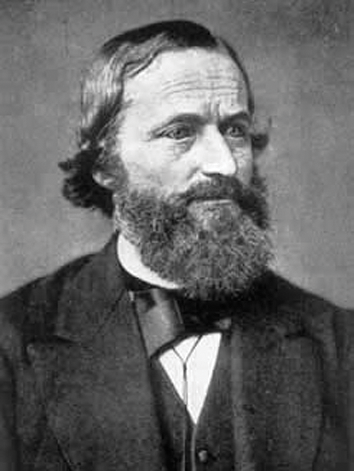
\includegraphics[width=\linewidth]{kirhof}
		\caption{Gustav Robert Kirchhoff 1824 – 1887}
		\label{fig:kirhof}
	\end{marginfigure} 
	
	Veliki napredak u istraživanju električnog strujanja u provodnicima zabilježen je 1847. godine, kada je Kirhof dedukcijom izveo i formulisao svoja dva zakona, koji spadaju u grupu temeljnih zakona klasične elektromagnetne teorije. \\
	Prvi Kirhofov zakon govori o  kontinuitetu električne struje, dok je drugi Kirhofov zakon matematički identičan sa zakonom da razlika potencijala između bilo kojih dviju tačaka ima istu vrijednost po svim putevima između njih. Ovi zakoni su vrlo korisni i mnogo su upotrebljavani u elektrotehnici. Imali su velikog značaja u njenom napretku i posebno su značajni za razvoj električnih krugova i mreža.
	
	\subsection{Uzajamno djelovanje naelektrisanih čestica}
	
	
	Elektrostatika je oblast fizike u kojoj se izučava elektricitet u mirovanju makroskopski posmatrano u odnosu na posmatračev referentni sistem, što znači da naelektrisanja smatramo statičkim (u miru) iako u njima postoji stalno kretanje naelektrisanih čestica.\\
	
	\begin{marginfigure}%
		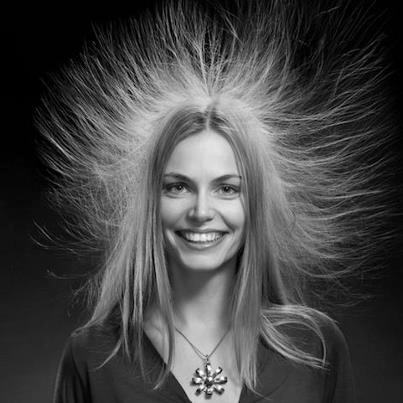
\includegraphics[width=\linewidth]{hair_static}
		\caption{Utvrđeno je da se neko tijelo može naelektrisati, ako se dodirne tijelom koje je već naelektrisano}
		\label{fig:hair_static}
	\end{marginfigure} 
	Fizikalna veličina koja opisuje stepen, odnosno mjeru naelektrisanosti neke čestice ili  tijela, zove se količina elektriciteta, količina naelektrisanja, ili električno opterećenje. Količina elektriciteta je skalarna, algebarska veličina, čija numerička vrednost govori, ili o višku, ili o manjku elektrona na nekom tijelu i označava se sa $ Q $ ili sa $ q $. Mjerna jedinica za količinu elektriciteta nosi naziv Kulon $ \textit{ C } $ francuskom fizičaru Kulonu.\\
	
	
	
	Rezultantno naelektrisanje atoma koji sadrži jednak broj protona i elektrona jednako je nuli. Kad neko tijelo sadrži višak elektrona, u odnosu na protone, kaže se da je negativno naelektrisano. U suprotnom, za tijelo koje ima manjak elektrona, kaže se da je pozitivno naelektrisano. Naelektrisanje $ q $, za koje se u literaturi susreću i nazivi: električno opterećenje, količina elektriciteta, električni naboj, jednako je:
	
	
	\begin{center}
		$ q= n e$,
	\end{center} 
	gdje je $ e $ elementarno naelektrisanje.
	%	\subsection{Elektroskop}

	\subsubsection{Elektroskop}
	
	
	\subsubsection{Zakon o očuvanju naboja}
	
	
	\subsection{Kulonov zakon}
	
	
	
	\subsection{Električno polje}
	
	
	\subsubsection{Jačina električnog polja}
	
	
	\subsubsection{Linije sile električnog polja}
	
	
	
	\subsubsection{Električno polje Zemlje}
	
	
	
	\subsection{Električni fluks}

	%	\subsection{Elektroskop}

	\include{elektrostatika/zakon-o-ocuvanju-naboja}
	\include{elektrostatika/kulonov-zakon}
	\include{elektrostatika/elektricno-polje}
	\include{elektrostatika/jacina-elektricnog-polja}
	\include{elektrostatika/linije-sile-elektricnog-polja}
	\include{elektrostatika/elektricno-polje-zemlje}
	\include{elektrostatika/elektricni-fluks}
	\include{elektrostatika/rad-u-elektricnom-polju}
	\include{elektrostatika/elektricni-potencijal}
	\include{elektrostatika/elektricni-napon}
	\include{elektrostatika/ekvipotencionalna-povrsina}
	\include{elektrostatika/kretanje-naboja-u-elektricnom-polju}
	\include{elektrostatika/elektricna-infuluencija}
	\include{elektrostatika/elektricni-kapacitet}
	\include{elektrostatika/elektricni-kondenzatori}
	\include{elektrostatika/vezivanje-kondenzatora}
	\include{elektrostatika/energija-elektricnog-polja}
	\include{elektrostatika/dielektrici-u-elektricnom-polju}
	\include{elektrostatika/elektricna-struja}
	
\printindex
\end{document}